\begin{figure}
	\centering
	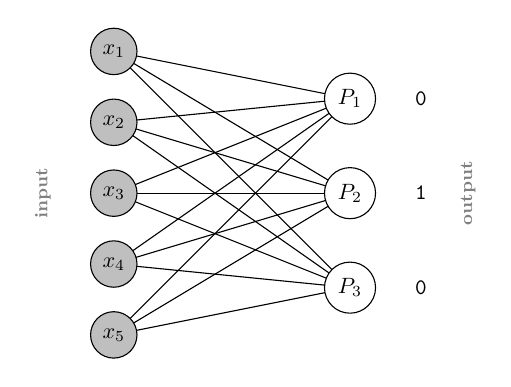
\begin{tikzpicture}[
		scale=0.6,
		every node/.style={scale=0.8}
	]

		\foreach \y in {-3,-1.5,0,1.5,3}{
			\foreach \yy in {-2,0,2}{
				\draw (-5,\y) -- (0,\yy);
			}
		}
	
		% input layer
		\foreach \y/\i in {3/1,1.5/2,0/3,-1.5/4,-3/5}{
			\node[circle,draw=black,fill=lightgray] at (-5,\y) {$x_{\i}$};
		}
		
		% rbf layer
		\foreach \y/\i in {-2/3,0/2,2/1}{
			\node[circle,draw=black,fill=white,align=center] at (0,\y) {$P_{\i}$};
		}
		\node at (1.5,2) {\texttt{0}};
		\node at (1.5,0) {\texttt{1}};
		\node at (1.5,-2) {\texttt{0}};

		\node[rotate=90,gray] at (-6.5,0) {\footnotesize \textbf{input}};
		\node[rotate=90,gray] at (2.5,0) {\footnotesize \textbf{output}};

	\end{tikzpicture}
\end{figure}